% CREATED BY DAVID FRISK, 2016
\chapter{Mise en Oeuvre}

Dans ce chapitre, nous allons parler des différentes étapes du projet de l'analyse du besoin à l'implémentation.

\section{Analyse du besoin}

Le premier point sur lequel nous nous sommes concentrés est l'analyse du sujet avant toute implémentation. 
Vous remarquerez que nous avons défini des fonctions externes comme étant internes pour des questions de personnalisation. Nous voulions faire un Shell à notre façon. 
\\D'abord, nous avons étudié le fonctionnement du "Bash". Cela nous a permis d'avoir une idée précise des fonctions d'un interpréteur de commandes et au final de faire le choix sur les fonctions à implémenter.
\\Niveau implémentation, il nous fallait une structure pour nous permettre de gérer les commandes et leurs paramètres et une deuxième (liste chainée) pour nous permettre de gérer les variables.
\\
{\fontfamily{pcr}\selectfont 
\\structure ParamCmd \{
\\  nom: chaine de caractères 
\\  argv: chaine de caractères
\\  argc: entier
\\\};
}
\\
{\fontfamily{pcr}\selectfont 
\\ structure Variables\{
\\   nom: chaine de caractères
\\   valeur: chaine de caractères
\\   suivant: structure variables // pointe vers l'adresse suivante
\\\} Variables;
}
\newpage
\section{Boucle de Fonctionnement du SHELL}
{\fontfamily{pcr}\selectfont 
\begin{lstlisting}[frame=single]

TANT QUE l'utilisateur ne ferme pas la session
FAIRE
Emettre un signe d'invite (prompt)
Lire la ligne courante
Traiter la commande entree
Executer la commande indiquee sur cette ligne
FIN 

\end{lstlisting}

}
\url{https://fr.wikipedia.org/wiki/Interpr\%C3\%A9teur\_de\_commandes}
\section{Choix du langage}
Nous avons choisi le C, du moins, il nous a été recommandé pour pouvoir programmer à bas niveau. Nous avions le choix entre utiliser les fonctions de la librairie standard et les appels systèmes. Notre choix s'est vite porté sur la librairie standard car elle a des fonctions déjà impléméntées que nous pouvions réutiliser. La principale raison du choix était la portabilité sur différentes architectures.
\section{Nos commandes}
\begin{figure}[h!]
\begin{center}
\centering 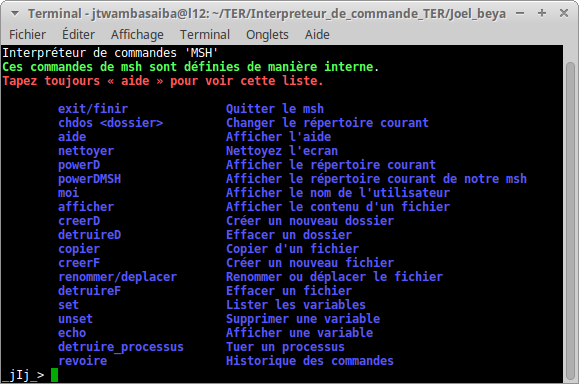
\includegraphics[scale=0.70]{figure/com.png}
\caption{\it Listes des commandes internes}
\end{center}
\end{figure}

\section{Fonctions majeures du programme }
Nous avons découpé le programme en plusieurs parties selon le fonctionnement d'un interpréteur de commandes.
\subsection{Prompt()}
L'interpréteur indique qu'il est prêt à recevoir une commande.
Nous avons implémenté un prompt dynamique pour permettre à l'utilisateur d'avoir plusieurs choix pour l'affichage de son prompt. Par exemple, l'utilisateur a le choix d'afficher les variables d'environnement ou encore de renommer le prompt comme il le souhaite. 
\\
\begin{lstlisting}[frame=single]
void prompteur()
\end{lstlisting}

\subsection{LireCommande()}
Elle nous permet de récupérer tout ce que l'utilisateur entre comme commande.
\\
\begin{lstlisting}[frame=single]
int  lire_commande(char* syf (resultat de la saisie 
de l'utilisateur))

\end{lstlisting}
\subsection{TraiterCommande()}
\\
Dans cette phase, nous traitons la commande comme le nom de la fonction l'indique. Nous récupérons le nom de la commande et ses arguments à travers les paramCmd.  Nous verifions si la commande existe dans notre fonction {\fontfamily{pcr}\selectfont void vérificateurCommande( saisie utilisateur ){}} dans laquelle on compare le nom de la commande et les fonctions que nous avons implémentées en utilisant "strcmp" de "string.h" de la librairie standard.
 
\begin{lstlisting}[frame=single]
int  traiter_commande(struct param_cmd* commande)
\end{lstlisting}
\subsection{ExecuterCommande()}
C'est la dernière phase avant le réaffichage du prompt ou la fin du programme selon la  commande entrée par l'utilisateur. A cette étape, nous gérons les processus et exécutons les commandes à travers "execvp" de la bibliothèque de la librairie standard "unistd.h" en recherchant par la même occasion le chemin . A travers cette même fonction, nous créons des processus fils. L'interruption par "CTRL+C" est désactivée si on se trouve dans le processus père et réactivée quand on est dans le fils. Aussi, notre fonction est capable d'exécuter une commande en arrière-plan à travers le "&"; C'est-à-dire, le père n'attend pas que le processus fils ait fini pour passer à autre chose.
\\
\begin{lstlisting}[frame=single]
int executer_commande() 
\end{lstlisting}


\section{Gestions des Signaux (SIGINT)}
SIGINT est envoyé lorsqu'un utilisateur presse la touche d'interruption du processus, typiquement Ctrl+C, dans notre cas. Alors nous avons absorbé le signal pour eviter que notre programme soit interrompu. Par contre on a fait en sorte d'interrompre les sous-programmes (ceux qui sont lancés dans le processus fils) quand l'utilisateur fait CTRL+C. Pour ce faire nous avons utilisé la structure "sigaction".

\begin{lstlisting}[frame=single]
sig.sa_flags = 0;
	sig.sa_handler = SIG_IGN;
	sigaction(SIGINT, &sig, NULL);
\end{lstlisting}

\section{Redirections}
\subsection{Rediriger la sortie dans un fichier : >}
On peut rediriger la sortie standard d'une commande vers un fichier (caractère ">"»). Le résultat de la commande sera placé dans le fichier au lieu de s'afficher sur l'écran. Exemple:  ls -l > toto.txt
Le résultat de ls -l ne s'affiche pas à l'écran, mais il est placé dans le fichier "toto.txt".
Pour cela, nous créons un fichier qui portera le nom du fichier destination entré par l'utilisateur et écrivons ensuite le résultat de la commande. Si le fichier existe déjà on l'écrase.
\\
\begin{lstlisting}[frame=single]
int redirection_Out(char* syf(resultat de la saisie de 
l'utilisateur), char* argv[], char* filename) 
\end{lstlisting}

\subsection{Ajouter la sortie à un fichier : > >} 
On veut parfois ajouter la sortie d'un programme à un fichier, sans effacer ce qui précède. Or, par défaut, si l'on tape plusieurs fois 
" ls -l > toto "
à chaque fois, le contenu antérieur du fichier toto est écrasé par le contenu ultérieur. 
Pour éviter cela, il existe l'outil de redirection > >.
\\Ainsi, si vous tapez "ls -l > > toto "
le fichier toto contiendra à la suite tout ce que vous a renvoyé la commande.
Dans ce cas, nous ouvrons le fichier s'il existe déjà, sinon on le crée et ajoute le résultat contrairement à la redirection simple qui écrase le fichier. 

\subsection{ Rediriger l'entrée: <} 
On peut aussi rediriger l'entrée standard d'une commande (caractère "<"). La commande lira alors le fichier au lieu du clavier. De cette façon, nous récupérons le résultat de la commande de droite puis nous la traitons avec la commande de gauche. Exemple: "afficher < message" va afficher le contenu de message.
\\
\begin{lstlisting}[frame=single]
int redirection_In(char* syf(resultat de la saisie de 
l'utilisateur), char* argv[], char* filename) {
\end{lstlisting}

\section{Communications entre différentes commandes à travers les tubes}
Le "|" permet de connecter deux processus. La sortie de la première instruction est utilisée en entrée de la deuxième et ainsi de suite. Le déclenchement de la fonction exécuterCommande dans la deuxième instruction dépendra donc de la première.

\section{Gestion des Variables}
Dans cette partie nous avons notre structure variables qui va nous permettre de manipuler des listes chainées et ainsi gérer nos variables. Par exemple, lorsqu'on fait val=16 , on affecte la valeur 16 à la variable val. 
\begin{lstlisting}[frame=single]
void ajout_Variable(char* nom_var, char val_var)
\end{lstlisting}

\section{Autocomplétion}
L'autocomplétion permet par exemple d'éviter de saisir complètement un nom de fichier. Il suffit donc de taper sur la touche "tab" dans l'interpréteur.Exemple avec toto.txt : L'appui sur la touche "tab" va afficher celui-ci sous réserve qu'il n'y ait qu'un fichier commençant par t. En cas de présence de plusieurs fichiers, il faut affiner en tapant la seconde lettre, puis éventuellement la troisième ...

Si nous trouvons une seule concordance, nous recopions le nom de fichier dans la chaîne readline, sinon rien ne se passe.

\section{Gestion de l'historique}

Nous créons un tableau pour nous permettre de stocker ce qui sera entré par l'utlisateur. Nous ouvrons  ensuite le fichier .myshell\_history qui enregistre les commandes saisies par l'utilisateur et nous lisons toutes les lignes et les stockons. Nous avons été aidé par la bibliothèque "readline/history.h", la bibliothèque "readline/readline.h" et "glob.h" que nous avons importé et nous avons utilisé quelques fonctions comme : 
\\
\begin{lstlisting}[frame=single]
void add_history (const char *string)
HIST_ENTRY * remove_history (int which)
void clear_history (void)
\end{lstlisting}


